\section{Experiment: Position-Length}

The position-length experiment by Cleveland and McGill involves the perception of five types of visualizations~\cite{cleveland_mcgill}. The visualizations are either grouped bar charts or divided bar charts (Fig.~\ref{fig:figure4_mlae}. Both types of graphs can show the same information but the elementary perceptual task is different. According to the theory by Cleveland and McGill, a grouped bar chart always involves the judgement of positions along a common scale. On the other hand, a divided bar chart might require length judgements in addition. Figure~\ref{fig:figure4_mlae} shows different charts of both types on the left. As identified by Cleveland and McGill, types 1, 2, and 3 involve the judgement of positions along a common scale while types 4 and 5 involve the measure of length. This means that this experiment does not just compare grouped versus divided bar charts but rather comparing position and length judgements.

For data generation we follow the same approach as in the original experiment. We generate pairs from ten values generated using Cleveland and McGill's equation

\begin{equation}
s_i = 10\times10^{(i-1)/12},\textnormal{~~~~~}i=1,...,10,
\end{equation}

with two different values for each pair. We then generate 8 other random values in the range of 10 and 93. These boundaries were chosen because we create rasterized visualizations using $100\times100$ pixel and want to stay in frame for a convolutional filter size of $5\times5$ in LeNet. We then visually encode the ten values as type 1--5. The paired quantities get marked by a single pixel. These are our quantities of interest and the task is to estimate the ratio of the smaller to the larger. We model this task as a single value regression. For type 4, we follow Cleveland and McGill's constraint that neither the top or the bottom of the marked quantities match to force length estimations rather than position.

We model this experiment as a single value regression task and ask networks to estimate the percentage of the smaller to the larger marked quantity in each visual encoding. The network first has to find the two marked quantities, then identify the smaller one, and finally estimate the ratio in comparison to the larger quantitiy. The 8 random quantities (which should be ignored by the network) push the number of possible permutations to a massive $9.20E+16$ and creates a very challenging problem.

Finally, we also train `multi' networks which include all five types resulting in an even bigger challenge.

\subsection{Hypotheses}

We proposed two hypotheses entering the elementary perceptual task experiment:

\begin{itemize}
  \item \textbf{H3.1} \textbf{Our networks can estimate all types equally well.} A grouped bar chart involves judging a position while a divided bar chart most likely (if not type 2) requires length judgements. Our rankings of elementary perceptual tasks do not yield a strong preference for either across all networks.
  \item \textbf{H3.2} \textbf{Trained `multi' networks work as well as individual trained networks.} Convolutional neural networks have massive numbers of trainable parameters. Their complexity allows them to learn different types of visual encodings in one training session. 
\end{itemize}


%\begin{figure*}[t]
%   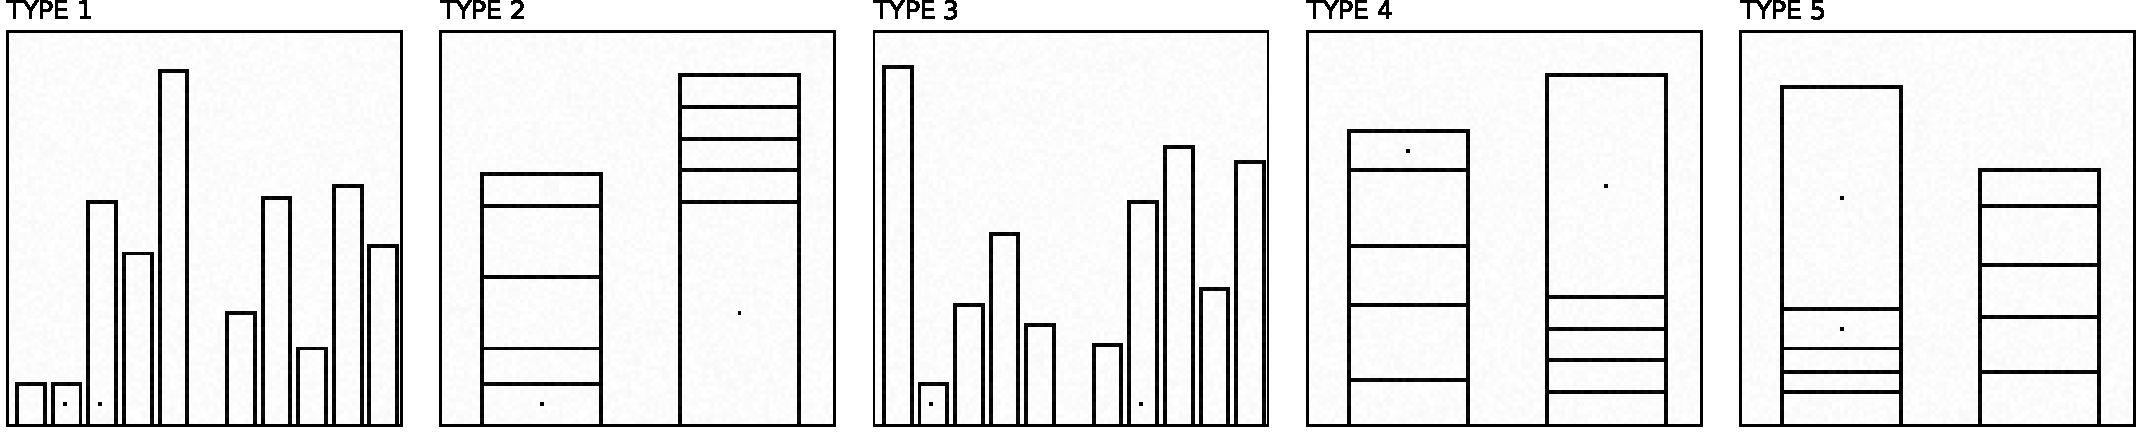
\includegraphics[width=\linewidth]{figure4_overview.pdf}
%   
%  \caption{\textbf{Position-Length Experiment.} (Not yet) Rasterized versions of the graphs of Cleveland and McGill's position-length experiment. The perceptual task involves comparing. the two dot-marked quantities across five different visual encodings of either grouped or divided bar charts. We evaluate which type of bar chart performs better with our neural networks as a combined classification and regression problem. The first task is to select which of the marked quantities is smaller (classification) and the second task is to specify how much smaller it is (regression).}
% \label{fig:position_length_experiment}
%\end{figure*}
%\begin{table}[h]
%\centering
%\caption{\textbf{Position-Length Experiment.} Rasterized versions of the graphs of Cleveland and McGill's position-length experiment. The perceptual task involves comparing the two dot-marked quantities across five different visual encodings of either grouped or divided bar charts. We evaluate which type of bar chart performs better with our neural networks. The two marked values are chosen from a set of ten pairs which defines the dual regression task. Since the other 8 values are chosen randomly, the parameter space for images of this experiment is massive.}
%\resizebox{\linewidth}{!}{
%\begin{tabular}{lllr}
% \toprule
% \multicolumn{2}{l}{~} & ~ & Permutations\\
% \midrule
% \raisebox{-.85\height}{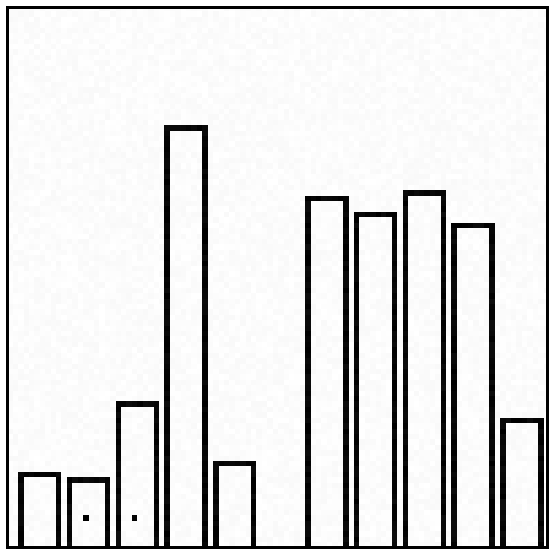
\includegraphics[width=.5in]{figure4_type_1.pdf}} & \makecell[tl]{Type 1: \emph{Grouped Bar Chart}\\~~~Perceptual Task: \emph{Position}\\~ \\~ \\} &~& \makecell[tr]{~\\ $9.20E+16$}\\
%
% \midrule
% \raisebox{-.85\height}{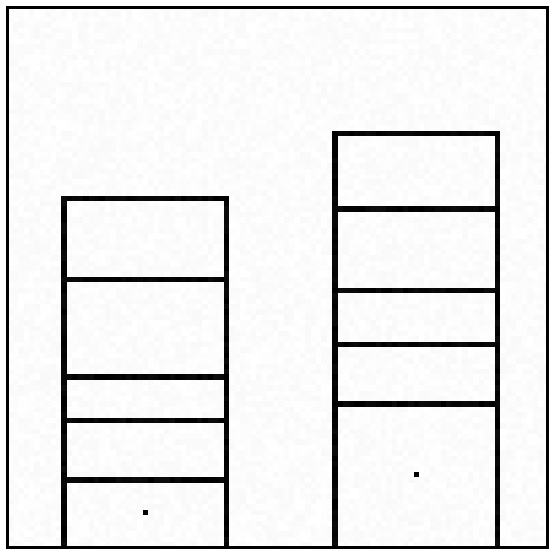
\includegraphics[width=.5in]{figure4_type_2.pdf}} & \makecell[tl]{Type 2: \emph{Divided Bar Chart}\\~~~Perceptual Task: \emph{Position}\\~ \\~ \\} &~& \makecell[tr]{~\\ $9.20E+16$}\\
% 
% \midrule
% \raisebox{-.85\height}{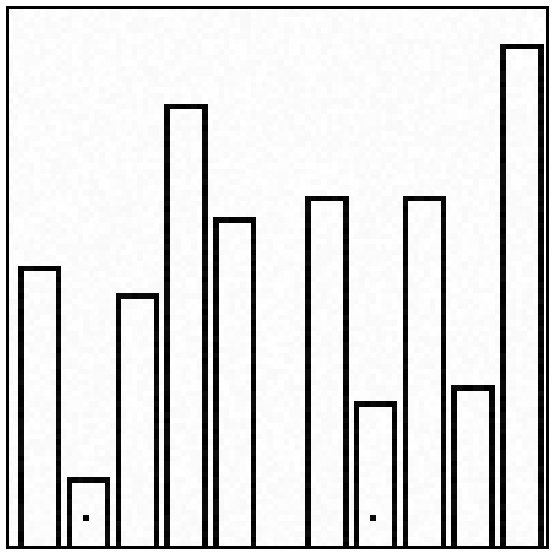
\includegraphics[width=.5in]{figure4_type_3.pdf}} & \makecell[tl]{Type 3: \emph{Grouped Bar Chart}\\~~~Perceptual Task: \emph{Position}\\~ \\~ \\} &~& \makecell[tr]{~\\ $9.20E+16$}\\
% 
% \midrule
% \raisebox{-.85\height}{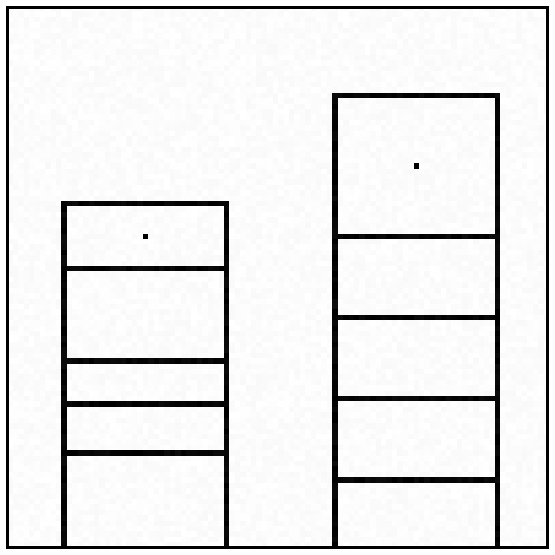
\includegraphics[width=.5in]{figure4_type_4.pdf}} & \makecell[tl]{Type 4: \emph{Divided Bar Chart}\\~~~Perceptual Task: \emph{Length}\\~ \\~ \\} &~& \makecell[tr]{~\\ $9.20E+16$}\\
% 
% \midrule
% \raisebox{-.85\height}{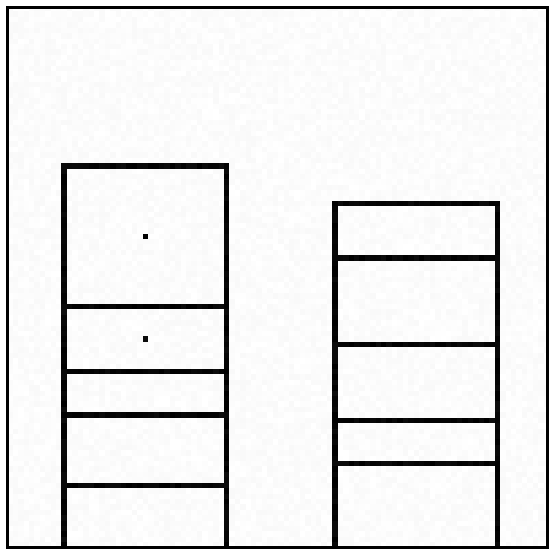
\includegraphics[width=.5in]{figure4_type_5.pdf}} & \makecell[tl]{Type 5: \emph{Divided Bar Chart}\\~~~Perceptual Task: \emph{Length}\\~ \\~ \\} &~& \makecell[tr]{~\\ $9.20E+16$}\\
%
% \bottomrule
%\end{tabular}
%}
%\label{tab:pos_length_parameters}
%\end{table}
%
%\subsection{Discussion}
%
%JT: Look at the relative difficulty of the tasks. In Cleveland and McGill, types 1-5 were post-ordered by their log error such that type 1 was easiest and type 5 was hardest. Is this still the case with our CNNs?

\subsection{Results}

\begin{figure}[!t]
  \centering
    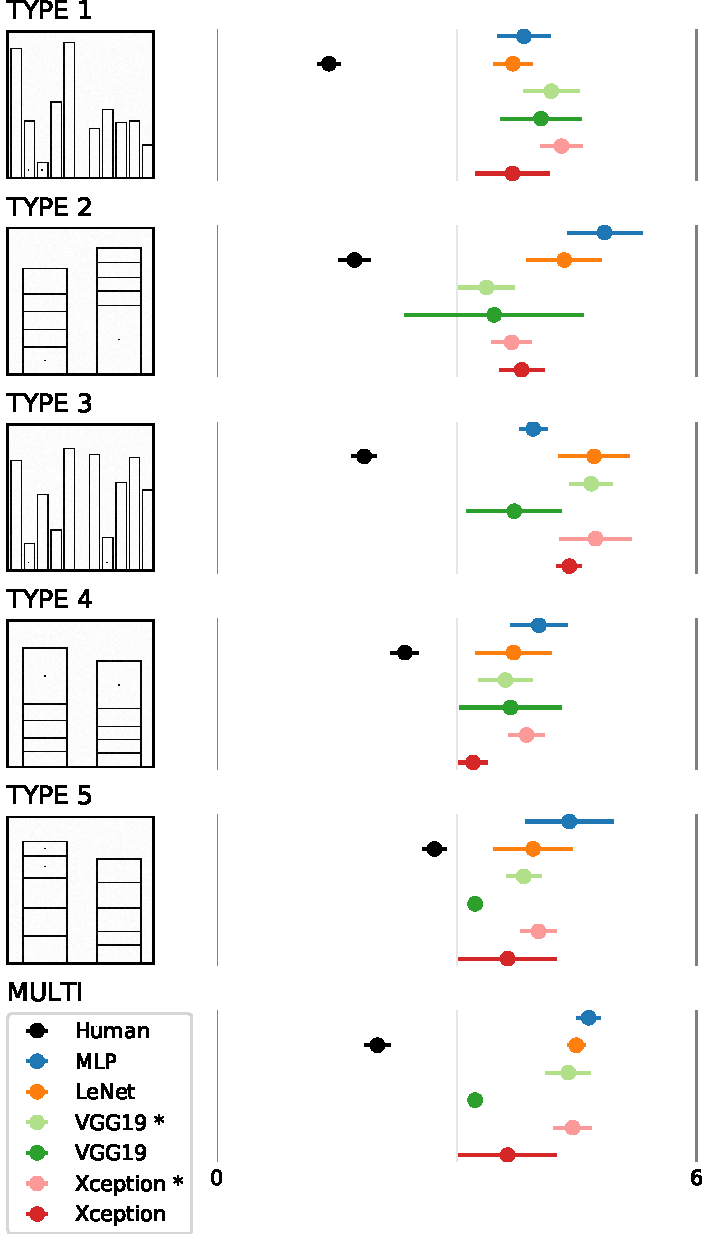
\includegraphics[width=\linewidth]{figure4_mlae_with_multi_and_humans_all.pdf}
  \caption{\textbf{Computational results of the position-length experiment.} \textit{Left:} Rasterized visualizations of type 1--5 for divided and grouped bar charts of Cleveland and McGill's position-length experiment. \textit{Right:} MLAE and $95\%$ confidence intervals for different regressors estimating the value of marked quantities in the visualizations. The VGG19 * and Xception * networks are using ImageNet weights. The top 5 rows represent networks trained on a single encoding while the last row shows `multi' networks which were trained on a random stream of types 1--5. We visually compare against human performance from the original experiment.}
  \label{fig:figure4_mlae}
\end{figure}

\noindent\textbf{Perceptual Performance.} In the original position-length experiment, Cleveland and McGill report that types 1-5 were post-ordered by their perceptual difficulty with type 1 being the easiest and type 5 the hardest. We report the average MLAE for each type across our networks (and total 56 runs per type) as follows: 
for type 1 $MLAE= 3.956 $ ($SD= 0.274 $),
for type 2 $MLAE= 3.952 $ ($SD= 0.441 $),
for type 3  $MLAE= 4.349 $ ($SD= 0.367 $),
for type 4 $MLAE= 3.668 $ ($SD= 0.256 $), and 
for type 5 $MLAE= 3.902 $ ($SD= 0.253 $). These distributions yield significance ($F_{4,25}=2.815, p<0.05$) but post hoc comparions show that really only type 3 and type 4 differ ($t_{10}=3.406, p<0.01$). This means that the networks do not prefer a certain type on average which leads us to \textbf{partially accept H3.1} and we do not replicate the same pattern as Cleveland and McGill in their human studies even though our networks' performance is clearly worse than their human baseline.
\\~\\
\noindent\textbf{`Multi' Network Performance.} In Cleveland and McGill's original position-length experiment, humans were asked to judge visualizations of types 1-5. In the bottom of Figure~\ref{fig:figure4_mlae} we average the human performances of types 1-5 to create a `multi' human. Similarly, when training our networks, we first limit each training to one stimuli. However, a `multi' network which learns types 1-5 simultaenously is closer to the human in the original user study. For our `multi' experiment, we record an average error across all classifiers of $MLAE=4.358$ ($SD=0.327$). We then compare against the average errors for all types, as reported above for perceptual performance. We reach significant differences ($F_{5,30}=3.454,p<0.05$). Post hoc comparisons yield significant differences between the `multi' experiment and type 4 ($t_{10}=3.716, p<0.01$) and also to type 5 ($t_{10}=2.467, p<0.05$). Since our the average MLAE is worse than all of type 1--5, and the distributions observe significant differences, we acknowledge that the `multi' task is harder for the networks than learning single types of encodings. This might relate to us fixing all other parameters of the experiment such as the number of early stopping epochs and the size of training data, however, we \textbf{reject H3.2}.


